\documentclass[12pt, a4paper]{article}
\usepackage[UTF8]{ctex}
\usepackage{amsmath}
\usepackage{amssymb}
\usepackage{amsthm}
\usepackage{geometry}
\usepackage{enumitem}
\usepackage{indentfirst}
\usepackage{caption}
\usepackage{fancyhdr}
\usepackage{booktabs}
\usepackage{titlesec}
\usepackage{draftwatermark}%水印
\usepackage{graphicx} % 导入图像的宏包、单图
% 页面布局设置
\geometry{top=2.54cm, bottom=2.54cm, left=3.18cm, right=3.18cm}

\SetWatermarkText{B站：布加拉提}
\SetWatermarkScale{0.4}

% 行距设置
\linespread{1.5}

% 段落设置
\setlength{\parindent}{2em}
\setlength{\parskip}{0.5em}

% 节标题格式设置
\titleformat{\section}{\normalfont\Large\bfseries}{第\chinese{section}章、}{1em}{}
\titlespacing{\section}{0pt}{2.5ex plus 1ex minus .2ex}{1.3ex plus .2ex}

% 定理环境设置
\newtheoremstyle{solution}
{}
{}
{}
{}
{\bfseries}
{、}
{1em}
{}
\theoremstyle{solution}
\newtheorem{sol}{解}

% 页眉页脚设置
\pagestyle{fancy}
\fancyhf{}
\fancyhead[C]{b站布加拉提整理（回忆版）b站甘茶w独家讲解}
\fancyfoot[C]{\thepage}

\rfoot{整理人：八方\\资源提供：考研乔瑟夫}
\lhead{
\includegraphics[width=0.06\linewidth]{p1.png}}
\rhead{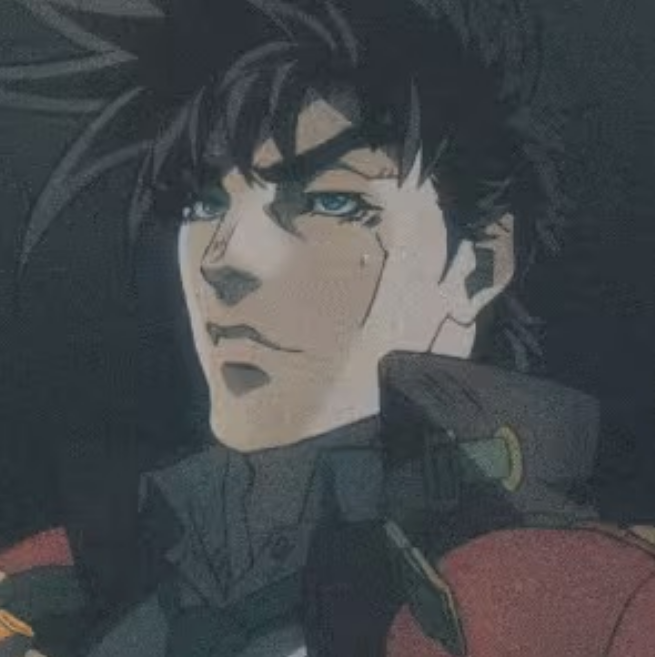
\includegraphics[width=0.06\linewidth]{p2.png}}
\renewcommand{\headrulewidth}{0.4pt}
\renewcommand{\footrulewidth}{0.4pt}

\begin{document}

\begin{center}
\Large\textbf{2002哈工大硕士考试试题：805物理光学}
\end{center}




\section*{一、选择题（共30分，每小题各三分）}
\begin{enumerate}
    \item 一束自然光通过偏振片，若两偏振片的偏振方向间夹角由\(\alpha_1\) 转到\(\alpha_2\) ，且不考虑吸收，则转动前后透射光强度之比为\_\_\_\_\_.\\(A)\(sin\alpha_1/sin\alpha_2\)  \quad
    (B)\(cos\alpha_1/cos\alpha_2\) \quad
    (C)\(sin^2\alpha_1/sin^2\alpha_2\) \quad
    (D)\(cos^2\alpha_1/cos^2\alpha_2\)
    \item 在夫琅和费单缝衍射实验中，对于给定的入射单色光，当缝宽变小时，除中央亮纹位置不变，各级衍射条纹\_\_\_\_\_.\\(A) 对应的衍射角变小\\(B) 对应的衍射角变大\\（C）对应的衍射角不变\\（D）光强也不变
    \item 两块平玻璃构成空气劈尖，左边为棱边，用单色平行光垂直入射。若上面的平玻璃以棱边为轴，沿逆时针方向作微小转动，则干涉条纹的\_\_\_\_\_.\\(A)间隔变小，并向棱边方向移动\\(B)间隔变大，并向远离棱边方向移动\\(C)间隔不变，并向棱边方向移动\\(D)间隔变小，并向远离棱边方向移动
    \item 在迈克尔逊干涉仪的一支光路中，垂直于光路放入折射率为\(n\)的透明介质薄膜后，测出两光束的光程差的改变量为一个波长，则薄膜的厚度是\_\_\_\_\_.\\(A) $\lambda/2$ \qquad (B)$\lambda/2n$ \qquad (C)$\lambda/n$ \qquad (D)$\lambda/2(n-1)$
    \item 在双缝干涉实验中，为使屏上的干涉条纹间距变大，可采取的办法是\_\_\_\_\_.\\(A)使屏靠近双缝\qquad(B)使缝的间距变小\qquad(C)把两缝的宽度稍微调窄\qquad(D)改用波长较小的单色光源
    \item 在真空中波长为$\lambda$的单色光，再折射率为\n 的透明介质中从A传播到B，若A,B两点的相位差为3\(\pi\) ,则此路径AB地光程差为\_\_\_\_\_.\\(A)1.5\(\lambda\) \qquad(B)1.5\(n\lambda\) \qquad(C)3\(\lambda\) \qquad(D)1.5\(\lambda/n\)
    \item 假设某一介质对空气的临界角是45°，则光从空气射向此介质时的布儒斯特角是\_\_\_\_\_.\\(A)\(tg^{-1}\sqrt{2}\) \qquad(B)tg^{-1}\sqrt{2}/2 \qquad(C)tg^{-1}(1/2)\qquad(D)tg^{-1}2
    \item 用波长为\(\lambda\)的单色光垂直照射折射率为\(n_2\)的劈尖薄膜，在薄膜上下介质的折射率分别为\(n_1\)和\(n_3\)，且\(n_1>n_2>n_3\),观察反射光干涉，从劈尖顶开始算起，第三条亮纹中心所对应的膜厚度为\_\_\_\_\_.\\(A)\(h=\lambda/n_1\)\qquad(B)\(h=\lambda/n_2\)\qquad(C)\(h=1.5\lambda/n_1\)\qquad(D)\(h=1.5\lambda/n_1\)
    \item 一衍射光栅对某一波长的垂直入射光在屏幕上只能出现零级和一级主极大，欲使屏幕上出现更高次的主级大，应该\_\_\_\_\_.\\(A)换一个光栅常数较小的光栅\qquad（B）换一个光栅常数较大的光栅\\（C）将光栅向靠近屏幕的方向移动\qquad（D）将光栅向远离屏幕的方向移动
    \item 一束光是自然光和线偏振光的混合光，让它垂直通过一偏振片，若以此入射光束为轴旋转偏振光，测得透射光强度最大值是最小值5倍，那么入射光束中自然光和线偏振光的光强比值是\_\_\_\_\_.\\(A)1/2\qquad（B）1/5\qquad（C）1/4\qquad（D）2/3
\end{enumerate}



\section*{二、简答题(共25分，每小题各5分)}
\begin{enumerate}
    \item 发生全反射的条件是什么？分析当线偏振光以大于临界角入射时，反射光的偏振状态
    \item 什么是光栅方程？简述它的物理意义。光栅有什么作用或用途？其性质用何参数可以描述？
    \item 什么是1/4拨片？它有什么作用？该器件是否能区分椭圆偏振光和部分偏振光？怎样区分？
    \item 两个频率相同，振动方向相互垂直的线偏振光叠加，其合成光有什么特点？是否产生干涉？要能产生干涉还应具备什么条件？
    \item 若使观察衍射光谱的最大衍射角固定不变，将光栅狭缝遮盖，光栅的分辨本领及自由光谱区有什么变化？
\end{enumerate}

\section*{三、计算题（共30分，每小题各10分）}

\begin{enumerate}
    \item 一束线偏振光$(\lambda=589.6nm)$垂直通过一块厚度为$1.618×10^{-2}mm$的石英晶片，晶片的折射率$n_o=1.54424,n_e=1.55335$,光轨沿x轴方向后，若入射光线偏振的振动方向与x轴成30°，决定出射光的偏振状态。
    \item 在双缝干涉实验中，波长$\lambda=550nm$的单色平行光垂直入射到缝间距$d=2×10^{-4}m$的双缝上，屏到双缝的距离$D=2m$,求
    \begin{enumerate}
         \item 中央明纹两侧的两条10级明纹中心的间距
         \item 用一厚度为$h=6.6×10^{-6}m$折射率为$n=1.58$的云母片覆盖一缝后，零级明纹将移动到原来的几级明纹处？
    \end{enumerate}
    \item 考虑三狭缝衍射屏，平行光垂直入射，假设三缝的宽度相等为$a=d/6$,两缝间距分别是d和3d/2.求衍射图样中：
    \begin{enumerate}
         \item 第一级主级大的\(\theta_1\)角是多少？
         \item 若在\(\theta=0\)方向的光强为I，问\(\theta/2\)方向上的光强为多少？
         \item 第一个衍射零级对应的是第几级主级大？
    \end{enumerate}
\end{enumerate}
\section*{四、综合题(15分)}
\begin{enumerate}
    \item 请简述泰曼干涉仪的工作原理：说明它可能有什么用途；并根据你的理解，讨论其时空相干性.
\end{enumerate}
\end{document}
